\documentclass{beamer}
\usepackage[utf8]{inputenc}

\usepackage{utopia} %font utopia imported

\usetheme{Madrid}
\usecolortheme{default}

%------------------------------------------------------------
%This block of code defines the information to appear in the
%Title page
\title[Domain-Driven-Design] %optional
{An Automated Form Building Application Based on Domain-Driven-Design}

%\subtitle{A short story}

\author[Arthur, Zhefei Chen] % (optional)
{Zhefei Chen}
%{A.~B.~Arthur\inst{1} \and J.~Doe\inst{2}}

\institute[NJU] % (optional)
{
  Department of Computer Science
  of Nanjing University
}

\date[I2EC 2020] % (optional)
{\today}

%\logo{
\includegraphics[height=1.5cm]{lion-logo.jpg}}

%End of title page configuration block
%------------------------------------------------------------



%------------------------------------------------------------
%The next block of commands puts the table of contents at the 
%beginning of each section and highlights the current section:

\AtBeginSection[]
{
  \begin{frame}
    \frametitle{Catalog}
    \tableofcontents[currentsection]
  \end{frame}
}
%------------------------------------------------------------


\begin{document}

%The next statement creates the title page.
\frame{\titlepage}


%---------------------------------------------------------
%This block of code is for the table of contents after
%the title page
\begin{frame}
\frametitle{Catalog}
\tableofcontents
\end{frame}
%---------------------------------------------------------


\section{What is Domain-Driven-Design}

\begin{frame}
\frametitle{From Domain Model to Work}
\begin{block}{The Definition of Domain}
A rigorously organized and selective abstraction of knowledge.
\end{block}
\begin{alertblock}{The Definition of Domain-Driven-Design}
The structure and language of software code (class names, class methods, class variables) should match the business domain.
\end{alertblock}
\begin{examples}
If a software processes loan applications, it might have classes such as LoanApplication and Customer, and methods such as AcceptOffer and Withdraw.
\end{examples}
\end{frame}
\begin{frame}
\frametitle{The Utility of a Domain Model in Domain Driven Design}
\begin{itemize}
    \item <1-> The model and the heart of the design shape each other.
    
    Which means changes of the model will lead to the changes of the design of the software system.
    
    \item <2-> The model is the backbone of a language used by all team members.
    
    Using a specialized language tailored for this model can erase the difficulty in the communication between engineers and the project manager(Assume that the project manager knows exactly what the requirements are).
    
    \item <3-> The model is distilled knowledge. 
    
    It reduces the efforts that engineers need to make to communicate with each other because model contains the condensed knowledge we hold about a domain and its components.
\end{itemize}
\end{frame}

\section{Apply DDD in our Form Building App}

\begin{frame}
\frametitle{The Composition of a Form Building App}

\begin{itemize}
    \item The Basic Knowledge About a Form Building App
    \item The Domain Model Design \& Former Framework
    \item The New Framework Applied in Development
\end{itemize}

\end{frame}

\begin{frame}
\frametitle{The Basic Knowledge About a Form Building App}

\begin{itemize}
    \item Main Function: Constructing \& Storing Forms
    \item Special Requirement: Customers may frequently change their ideas, and the form they need has to be modified along with the changes of ideas.
\end{itemize}

\end{frame}

\begin{frame}
\frametitle{The Domain Model Design \& Former Framework}
\begin{itemize}
    \item <1-> The Core Knowledge: Forms, Customers and Engineers
    \item <2-> The Domain Model Design: We need to define Classes for Forms, Customers and Engineers, and methods for creating \& storing forms and data.
    \item <3-> Traditionally we use Java code to define classes, and this method works in most situations. At first we treated the domain model of Form the same as Customer's and engineer's, so we logically define different Form Classes since there could be different kinds of forms facing different requirements. 
\end{itemize}

\end{frame}

\begin{frame}{Former Framework}
We recognize the domain model of form as classes defined by Java Code.
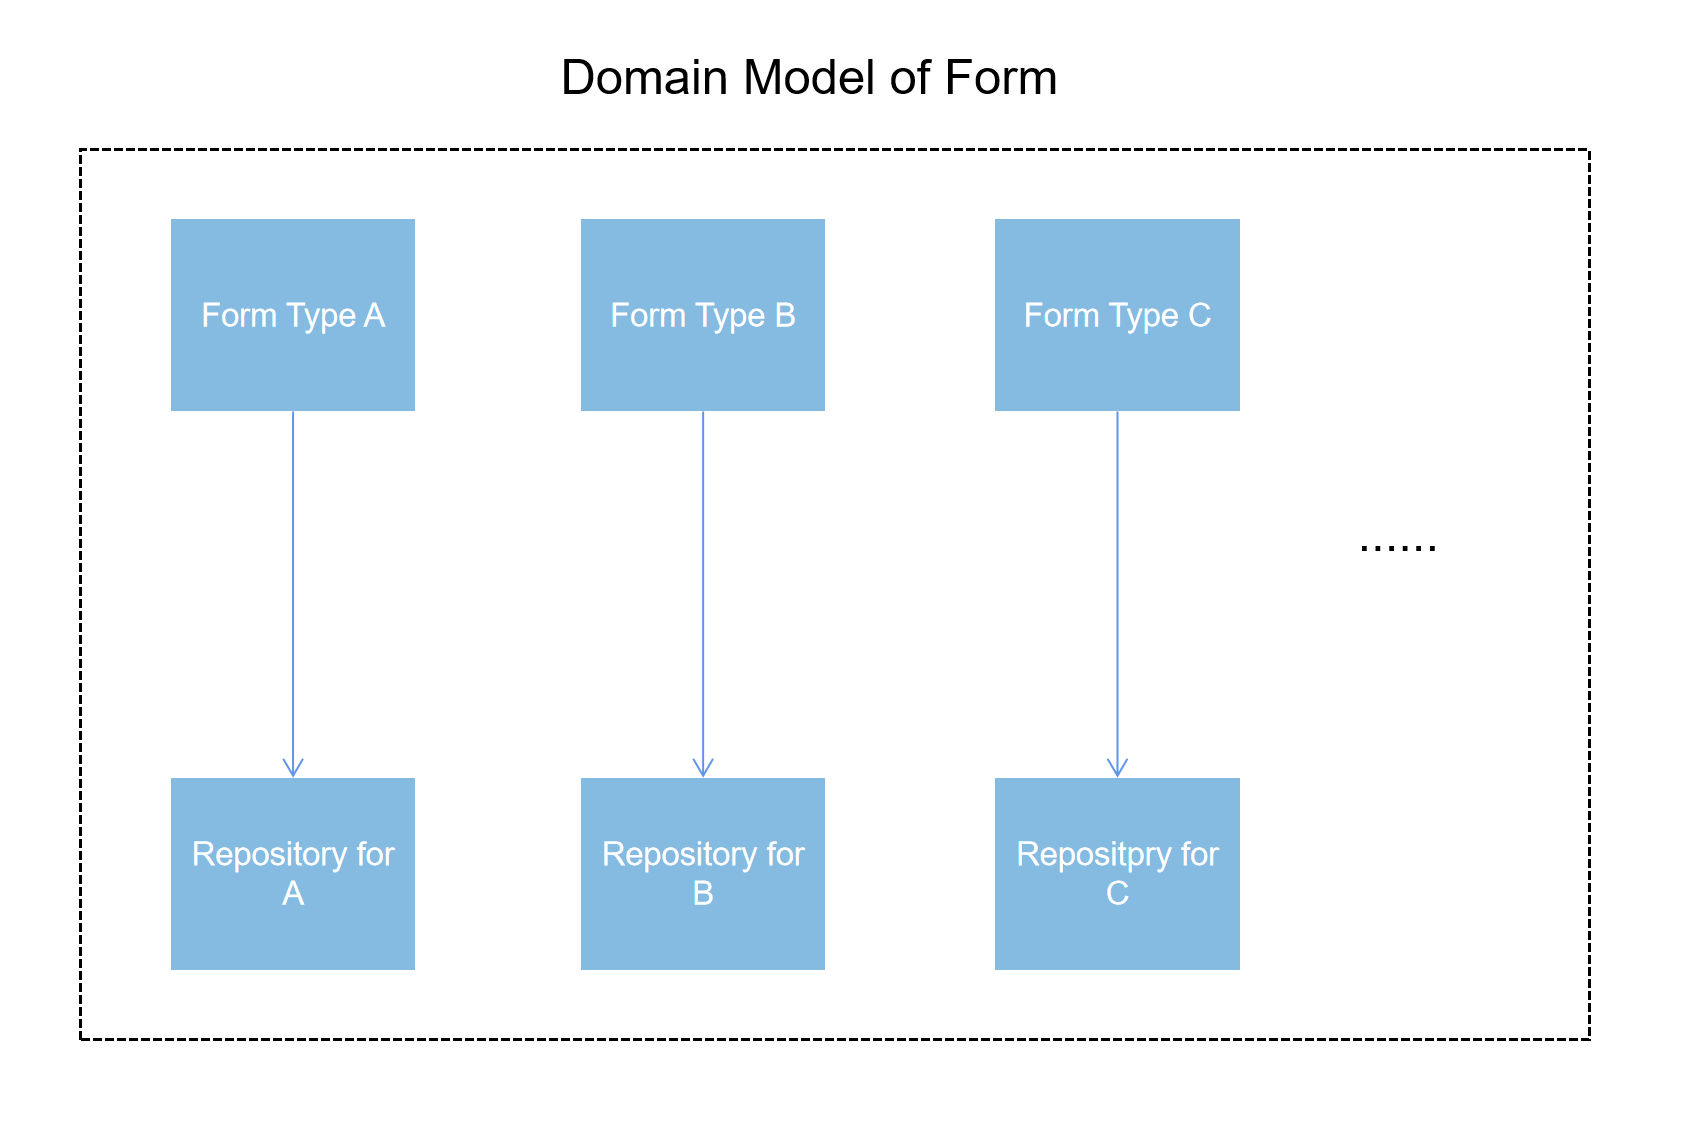
\includegraphics[width=0.9\linewidth]{domainform1.png}
\end{frame}

\begin{frame}{Former Framework}
Eventually we think in the following way that engineers passively create or modify the classes defined for forms to satisfy the changing requirement.
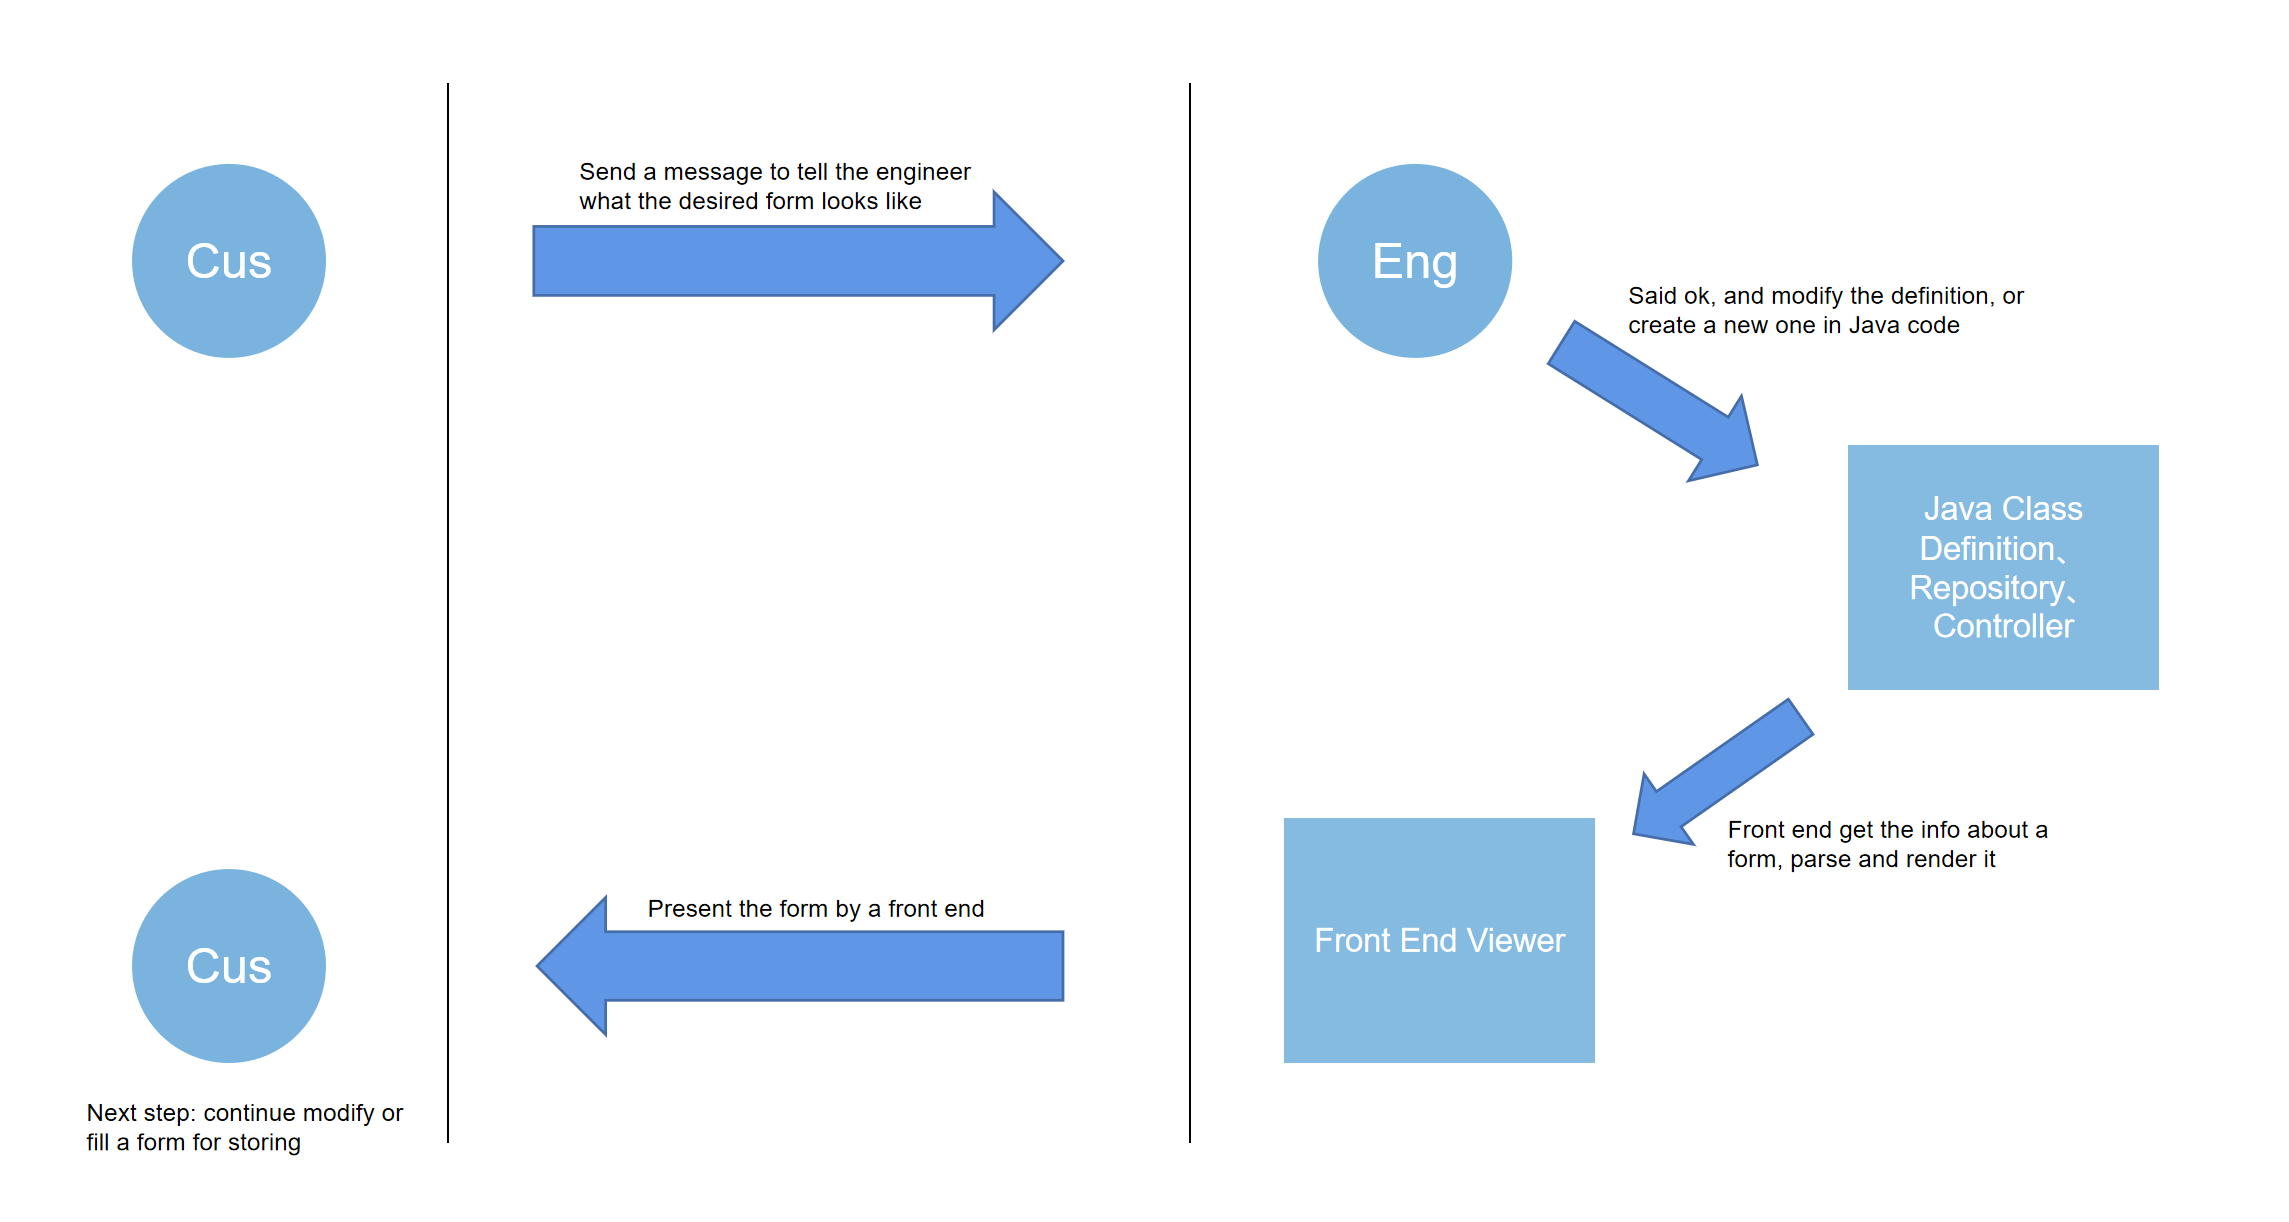
\includegraphics[width=0.9\linewidth]{former framework1.png}
    
\end{frame}

\begin{frame}{Former Framework}
The system came as following:
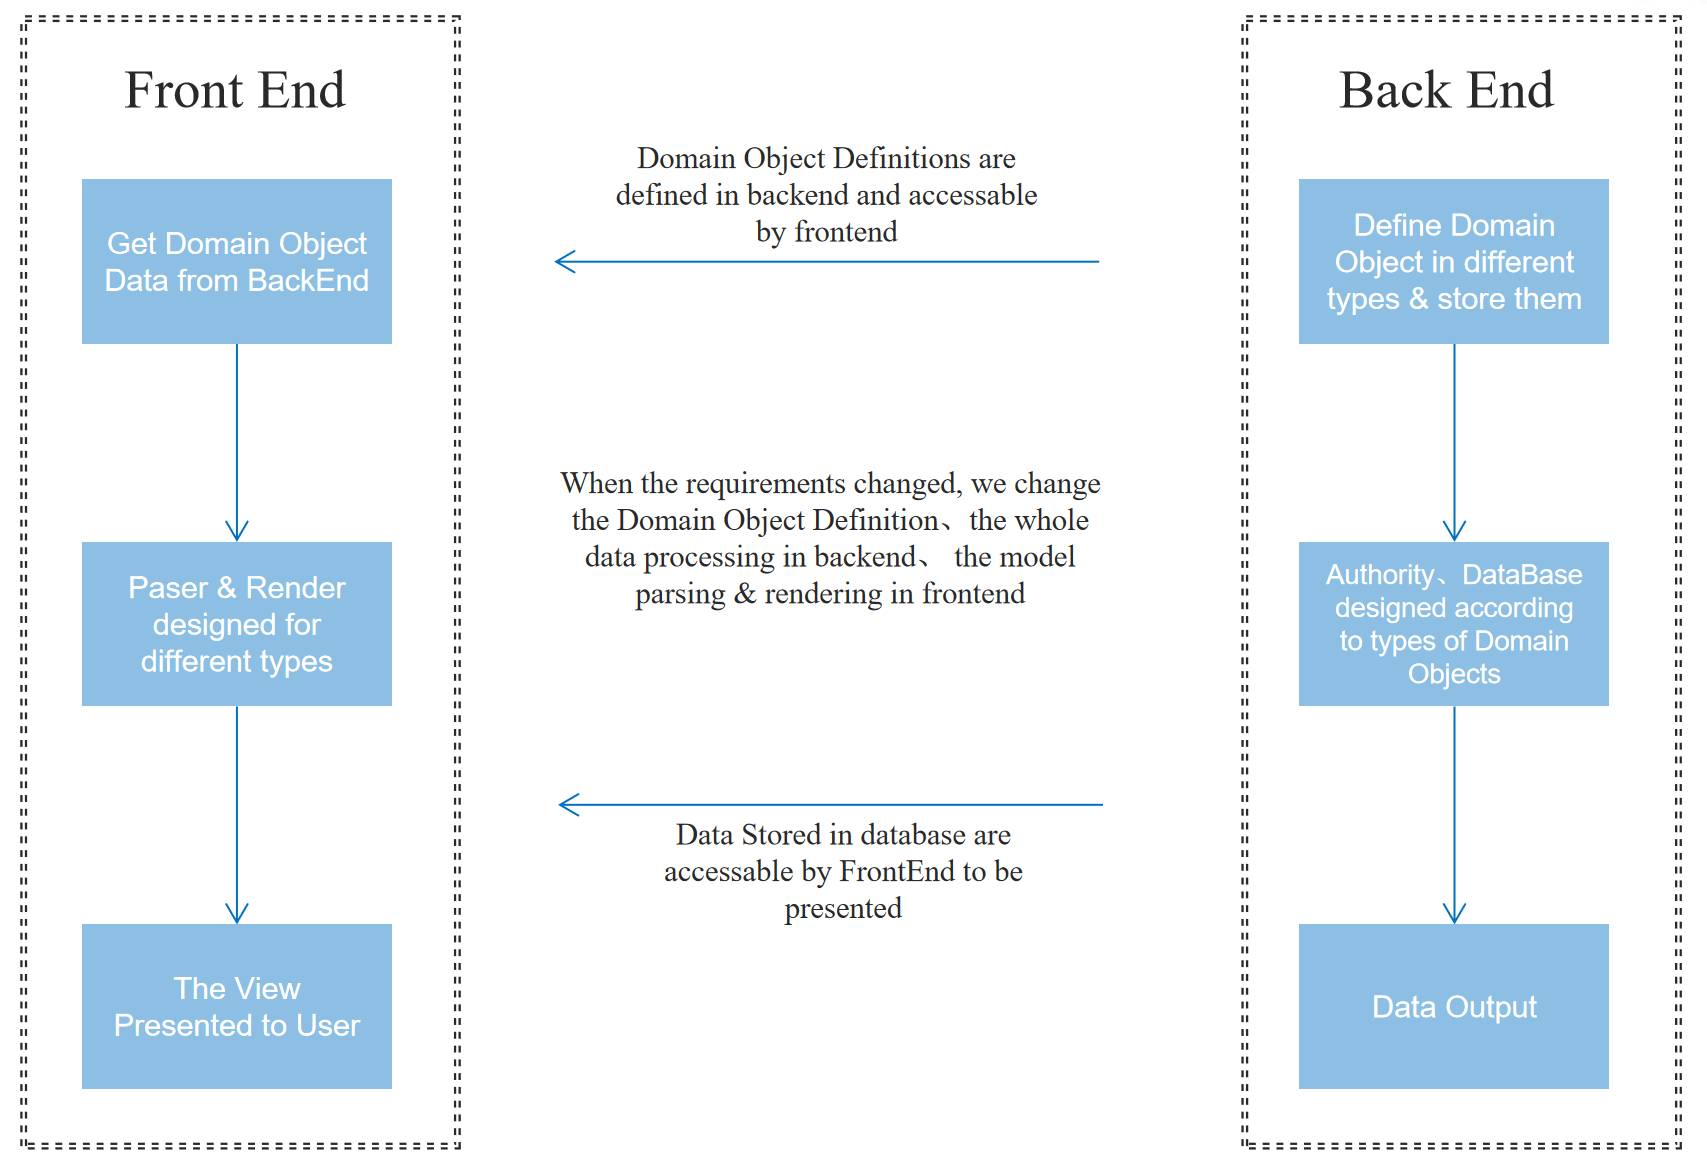
\includegraphics[width=0.9\linewidth]{former framework2.png}
\end{frame}

\begin{frame}
\frametitle{The New Framework Applied in Development}
\begin{itemize}
    \item <1-> Problem: How to reduce the cost brought by changes of requirements
        
    \item <2-> What if we think in a different way when designing the domain model of form?
    
\end{itemize}
\end{frame}

\begin{frame}{The New Framework Applied in Development}
We separate a form definition into different attributes, thus the process of defining a kind of form becoming the combination of attributes.
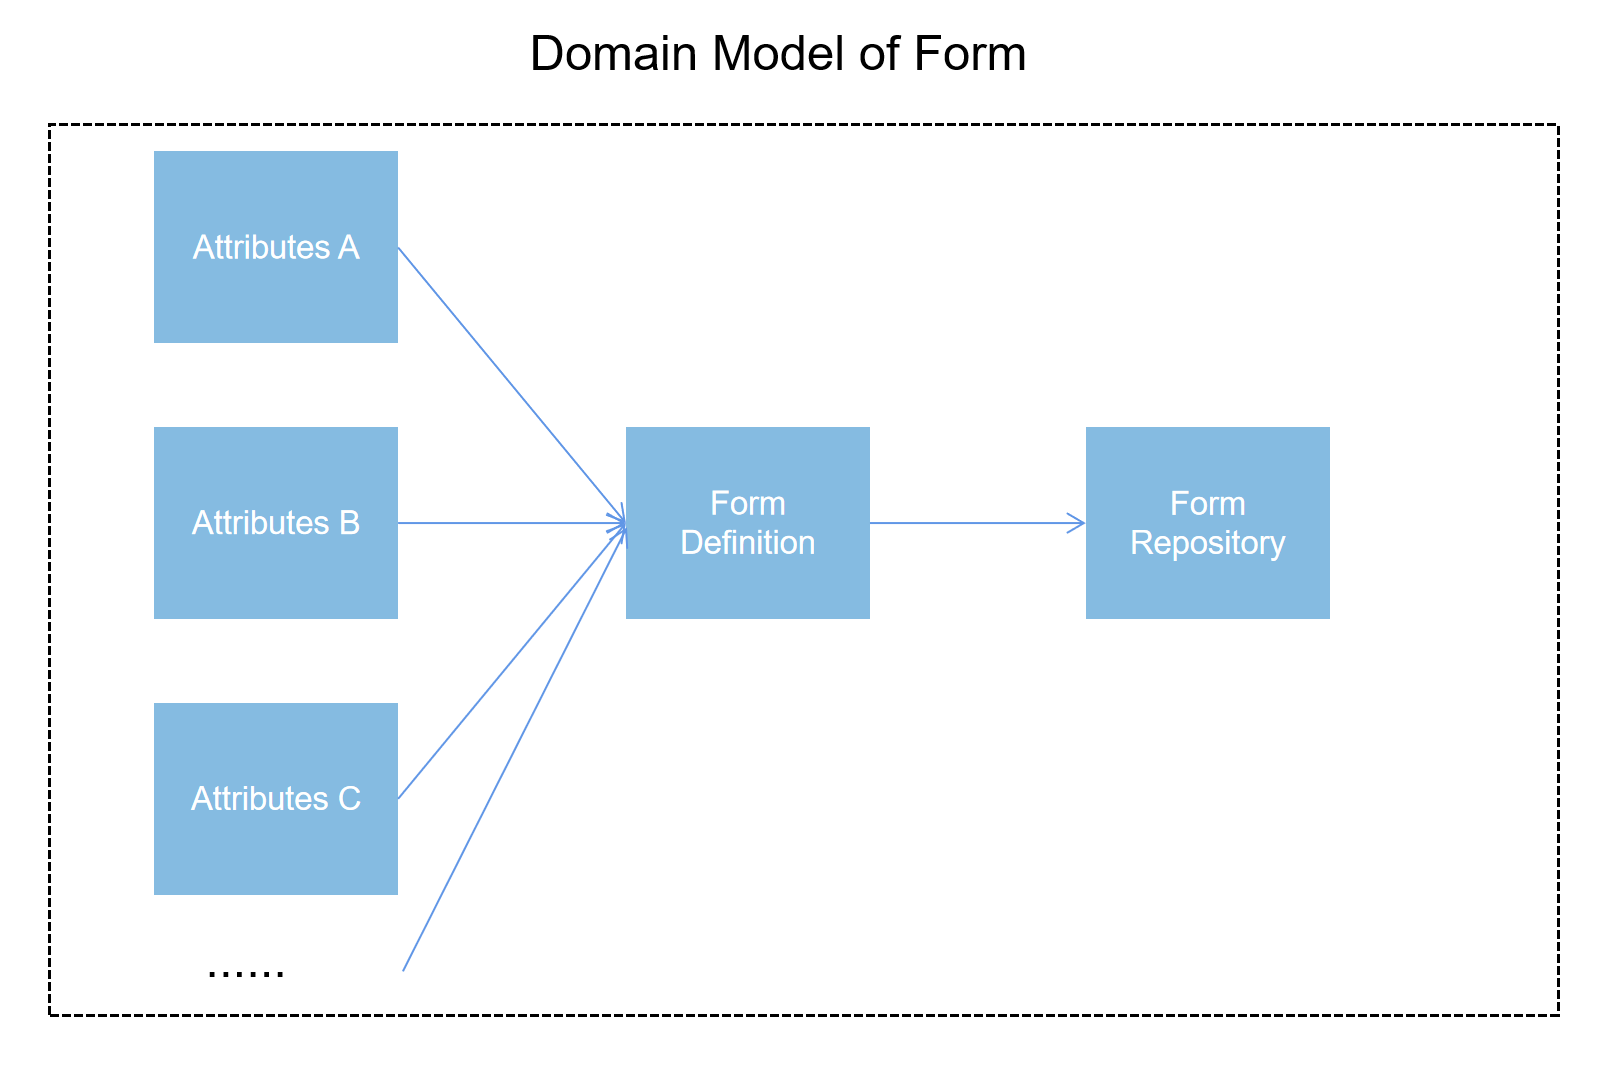
\includegraphics[width=0.9\linewidth]{domainform2.png}
\end{frame}

\begin{frame}{The New Framework Applied in Development}
And the whole process becomes that customer constructs a form he needs on his own, engineers are only responsible for storing the form designed correctly.
    
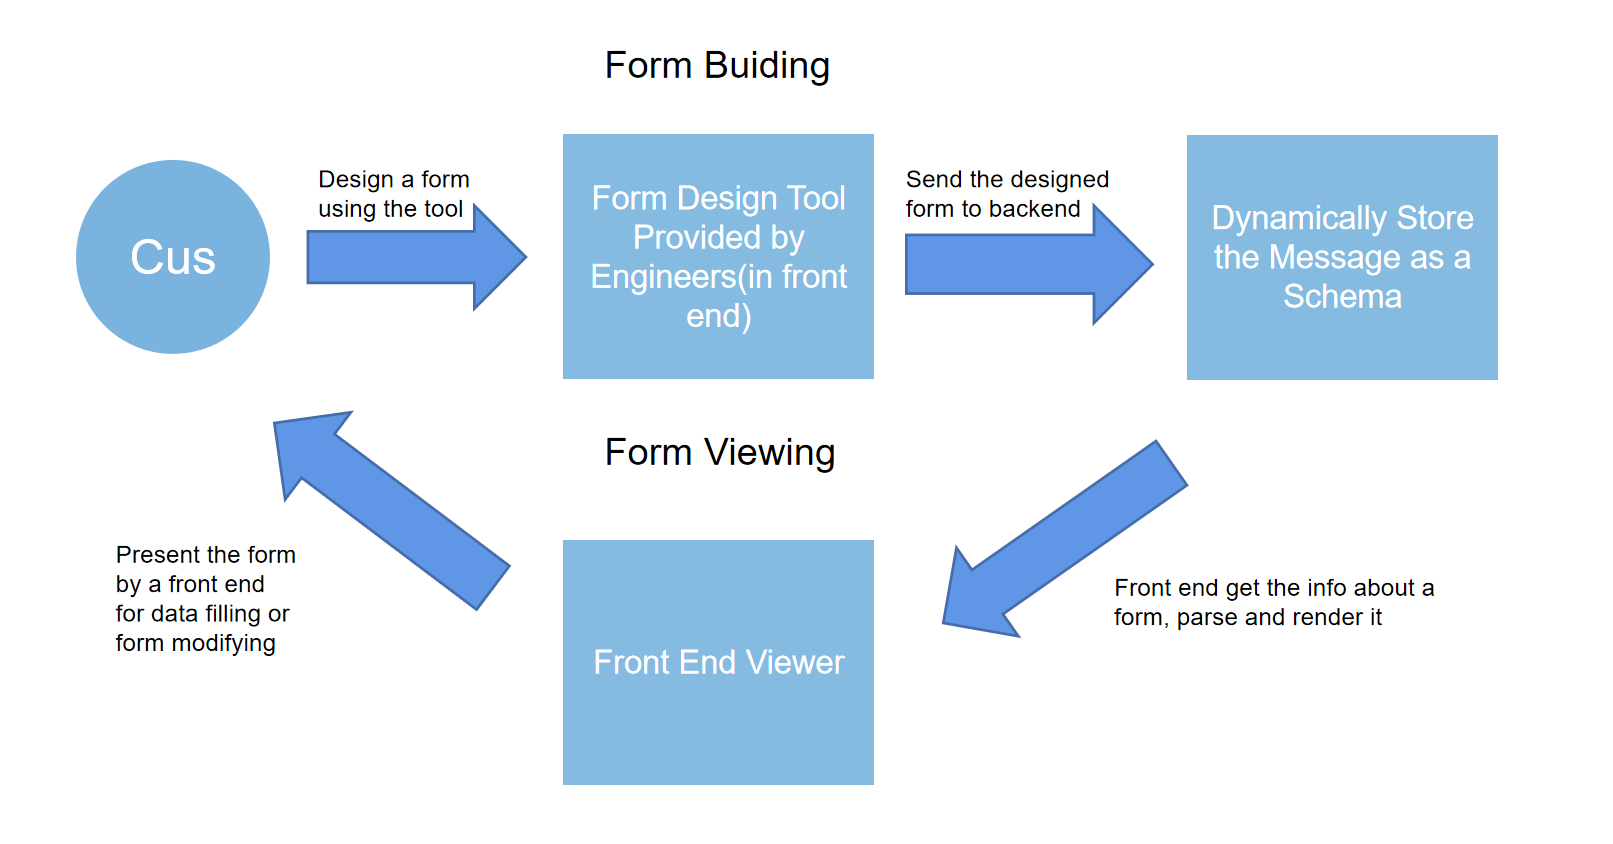
\includegraphics[width=0.9\linewidth]{framework3.png}
\end{frame}

\begin{frame}{The New Framework Applied in Development}
The new framework appears: 

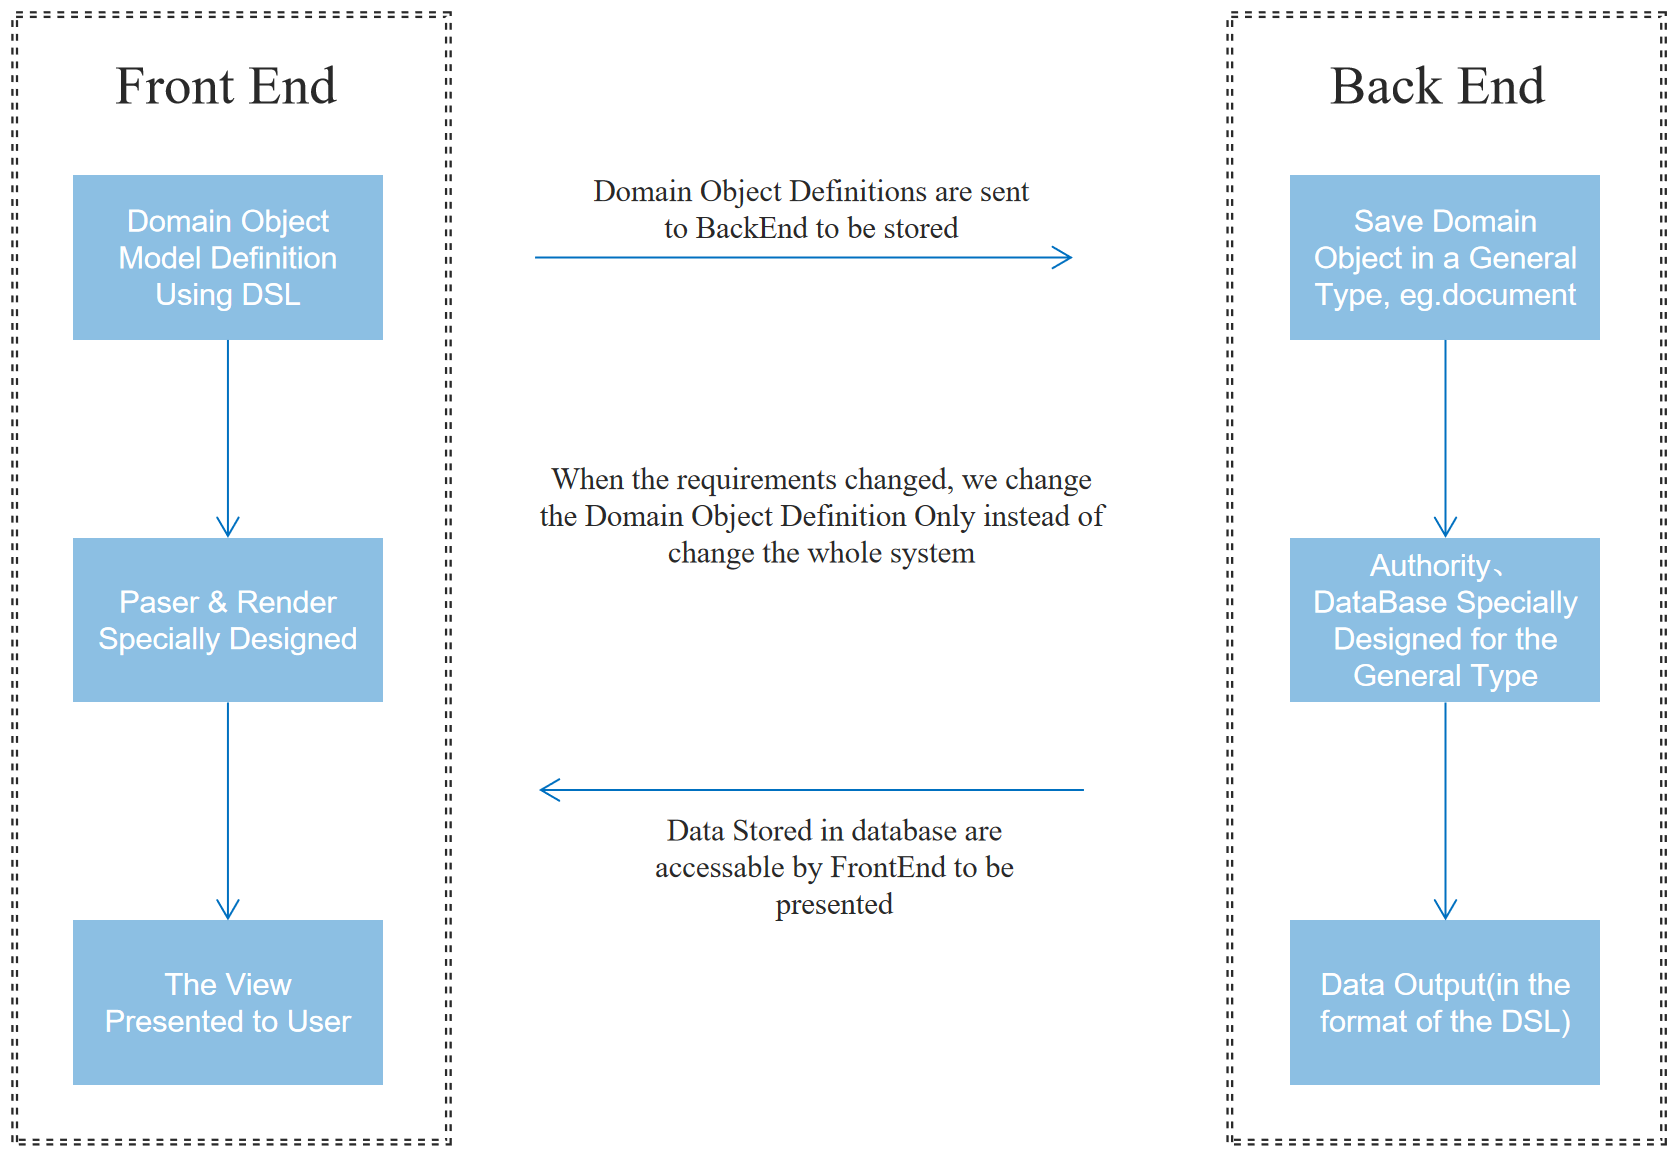
\includegraphics[width=0.9\linewidth]{framework4.png}
    
\end{frame}

\section{Conclusion: Inspirations of DDD and Future Work}

\begin{frame}
\frametitle{Conclusion: Inspirations of DDD}
\begin{itemize}
    \item <1-> Applying Domain-Driven-Design helps us build project in a more systematical way, which explicitly explains what a software is made for and what it consists of.
        
    \item <2-> A good design of Domain Model can reduce software engineers' burden when changes of requirements occur.
    
    \item <3-> We can integrate Domain-Driven-Design with a specified DSL to come up with a specially designed framework to satisfy the complexity of requirements.
\end{itemize}
\end{frame}

\begin{frame}{Future Work}
Though we improved the performance of the app by change the details of domain model, there are still some problems need to do.
\begin{itemize}
    \item <1-> Using Json Schema as a DSL has its demerits when we need to build a large form with many options. In that situation, the schema text of a form could be to long to be accepted by engineers. 
    
    Solution: We are now working to develop a specified DSL to overcome the drawbacks of Json Schema.
        
    \item <2-> Now we have a front end for form creating and filling, a back end for storing and searching data, but the Authorization part of back end is not finished yet, we still need to work on to complete the whole framework for a DDD Form Building App.
    
\end{itemize}

\end{frame}

\begin{frame}{Future Work}
Ideally we will finally present a DDD framework for this kind of Form building App, including not only the part of form constructing and storing, but also a complete back end with authorization and database access.
\end{frame}

\begin{frame}
    \centering{Thanks For Listening!
    
    Q\&A
    }
   
\end{frame}

\end{document}